\documentclass{deliverablereport}

\deliverable{UI}{ipython-kernels-basic}
\deliverydate{??/09/2016}
\duedate{01/09/2016 (M12)}
\author{Jeroen Demeyer, Markus Pfeiffer, Nicolas M. Thiéry}

\begin{document}
\maketitle
\githubissuedescription
\tableofcontents
\clearpage
\section{Screenshots}
\begin{figure}[ht]
  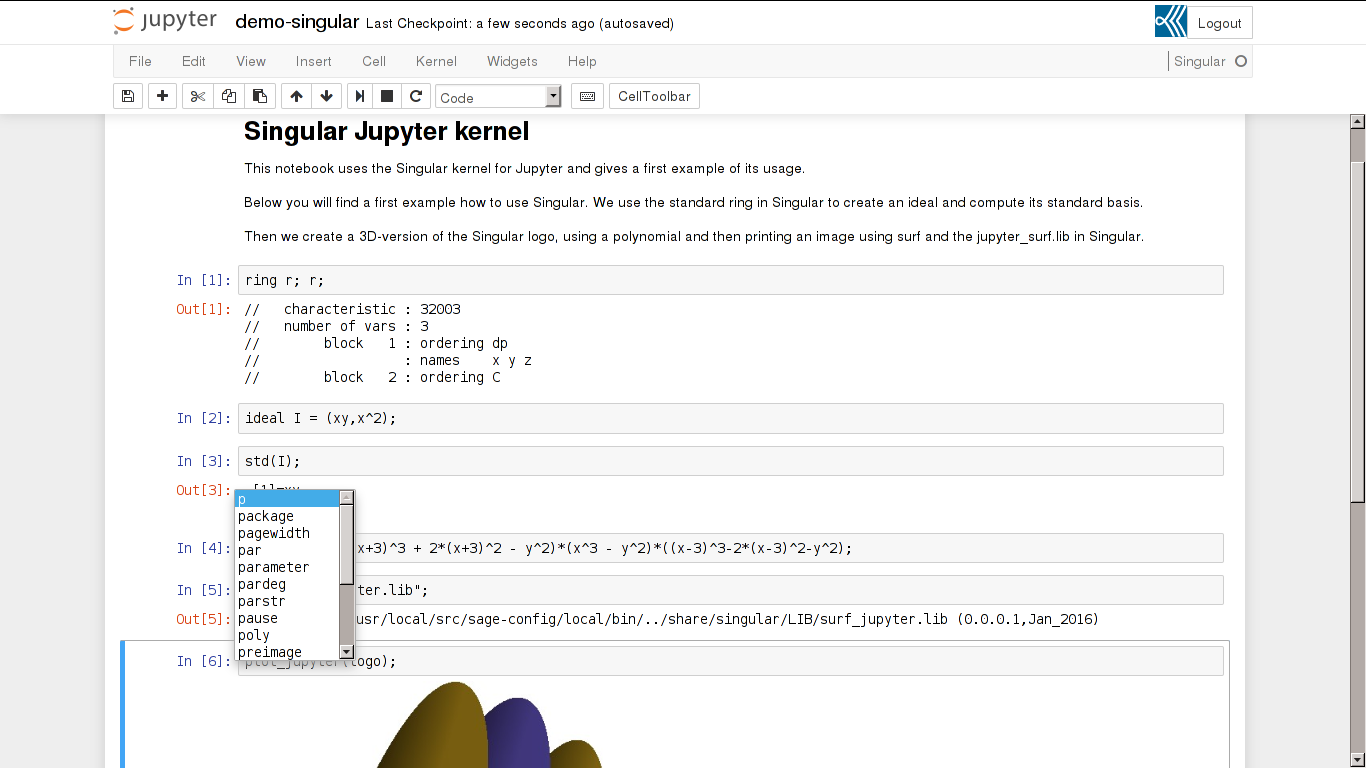
\includegraphics[width=140mm,trim={0 0 0 1px},clip]{singular.png}
  \caption{GAP's Jupyter kernel in action, showcasing ....}
\end{figure}
\begin{figure}[ht]
  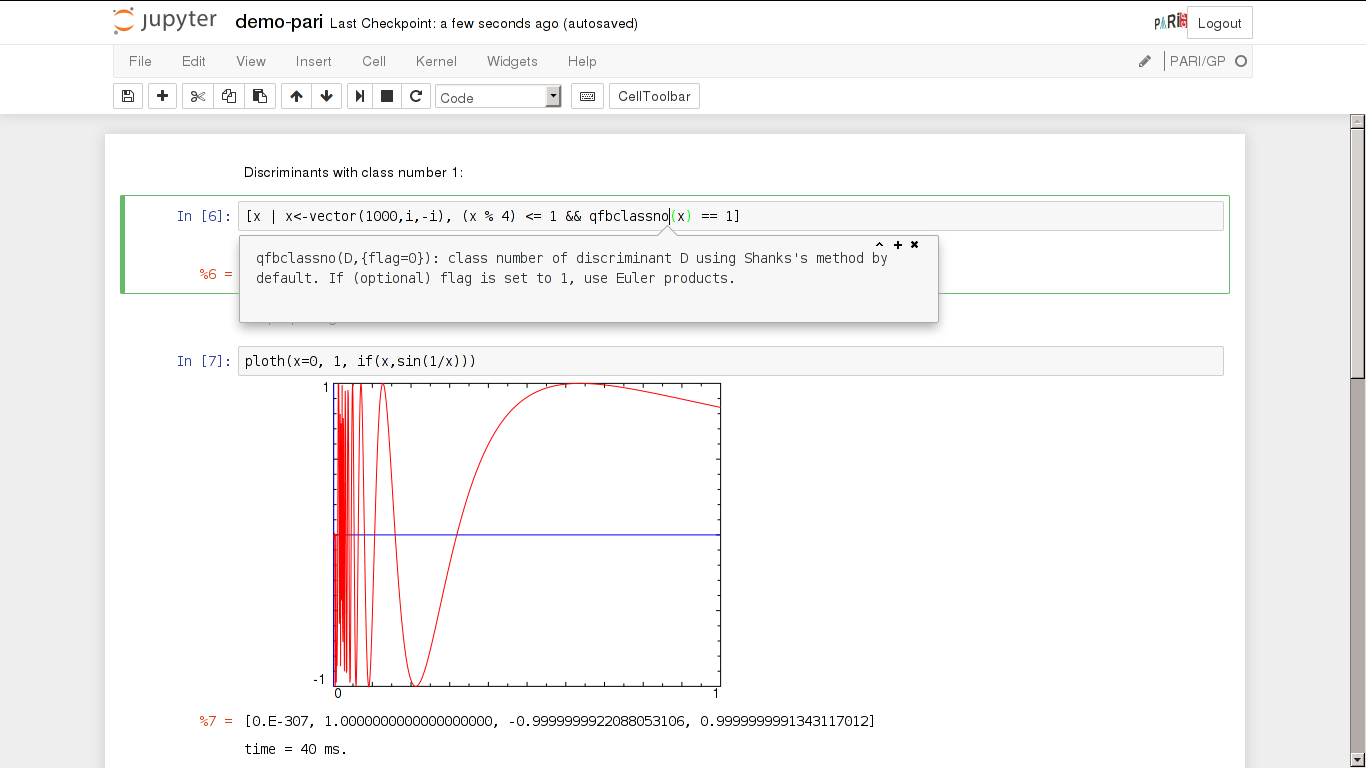
\includegraphics[width=140mm,trim={0 0 0 1px},clip]{pari.png}
  \caption{PARI/GP's Jupyter kernel in action, showcasing
    discriminant calculations, plotting and short help.}
\end{figure}
\begin{figure}[ht]
  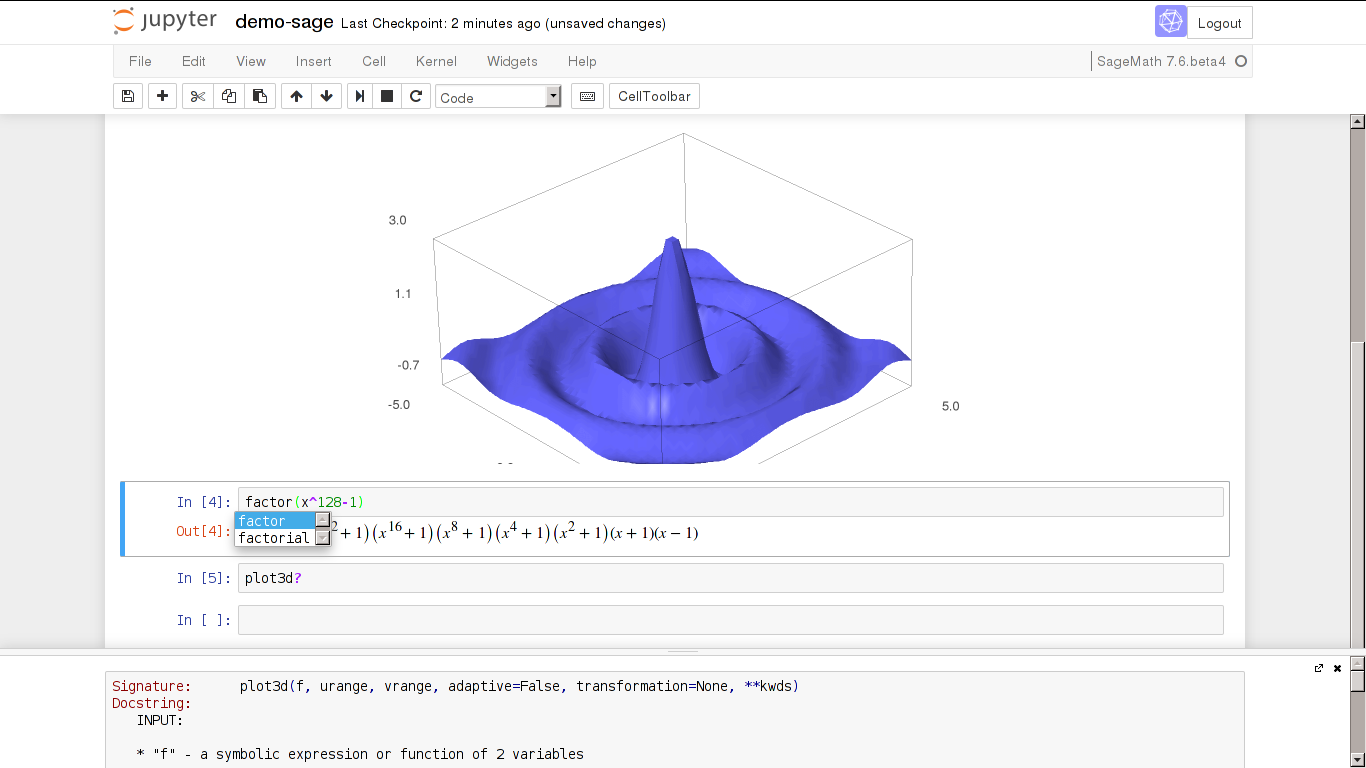
\includegraphics[width=140mm,trim={0 0 0 1px},clip]{sage.png}
  \caption{SageMath's Jupyter kernel in action, showcasing Mathjax
    typesetting, 3D plots, TAB-completion, documentation lookup.}
\end{figure}
\begin{figure}[ht]
  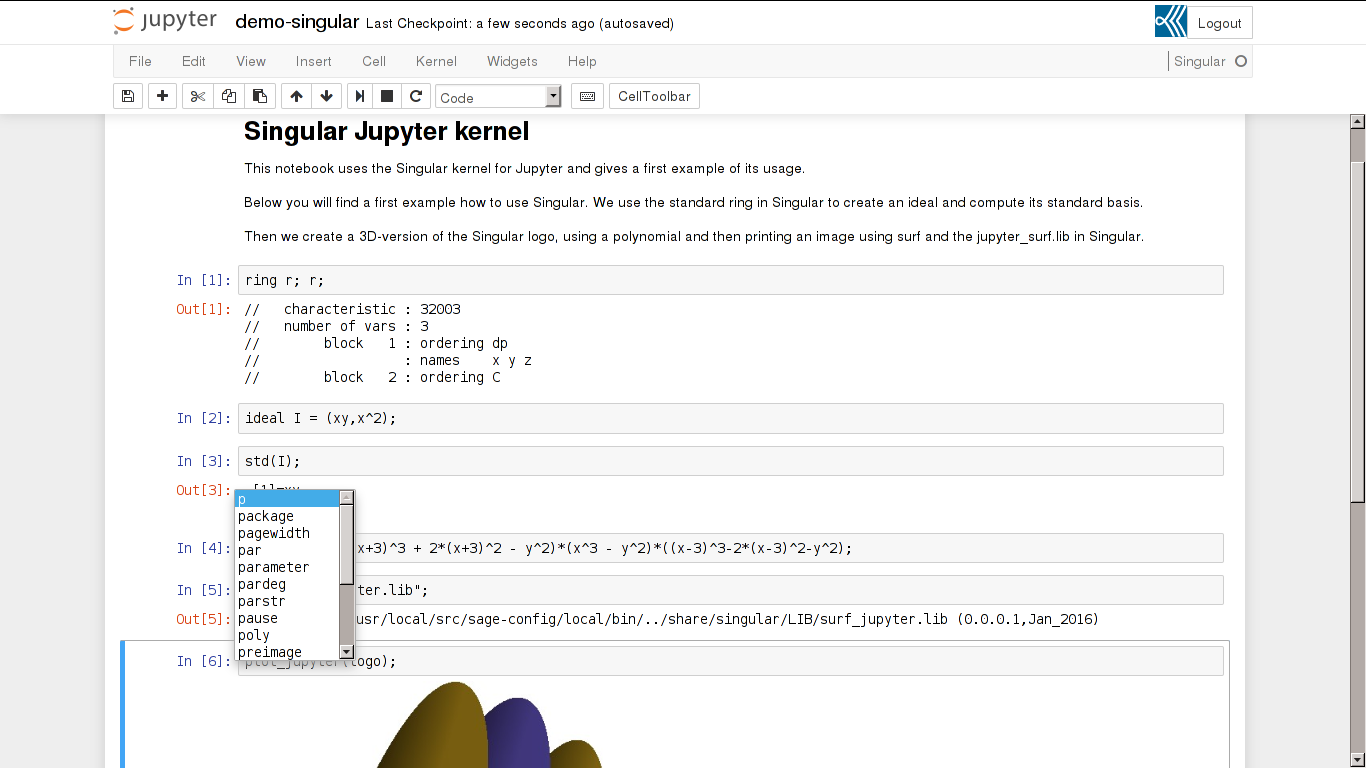
\includegraphics[width=140mm,trim={0 0 0 1px},clip]{singular.png}
  \caption{Singular's Jupyter kernel in action, showcasing polynomial
    calculations, 3D plots, and TAB-completion.}
\end{figure}
\clearpage
\end{document}

%%% Local Variables:
%%% mode: latex
%%% TeX-master: t
%%% End:
